\mychapter{Credential Relationship Binding Nullifier}

\noindent This pairing-free nullifier construction extends our MIMC-ABC system with efficient Sybil resistance while maintaining privacy. Beyond preventing credential reuse, the underlying zero-knowledge proof of multiplicative inverse enables a broader class of credential relationship predicates, enhancing the expressiveness of our anonymous credential system without sacrificing performance.

\section{Problem Statement and Motivation}
Anonymous Credential systems must balance user privacy with protection against Sybil attacks, where a malicious user creates multiple credentials. In our $\MIMCABC$ based Identity System, users possess a Master Credential containing a secret key $\k$ and may obtain multiple Context Credentials for different services or contexts. Each Context Credential contains a unique identifier $\ctx$ (e.g., $\mathcal{H}(\text{``DriverLicense''})$). During issuance, the system must ensure that each user receives at most one credential per context—without compromising privacy by revealing user identities.

Specifically, we need a privacy-preserving mechanism we need that creates a unique deterministic token (nullifier) for each user-context pair without compromising anonymity.

\subsection{Limitations of Existing Approaches}

Verifiable Random Functions (VRFs) offer a promising foundation for nullifier construction, but existing implementations have significant limitations:

\begin{itemize}
    \item \textbf{Standard VRF:} Traditional constructions expose the user's public key during verification, breaking unlinkability between credential uses~\cite{hutchison_verifiable_2005}

    \item \textbf{MPC PRF} Systems like CanDID~\cite{maram2021candid} use secure multi-party computation to preserve anonymity but introduce substantial overhead and prevent dynamic nullifier generation.

    \item \textbf{Pairing-based Approaches:} Recent constructions like UTT~\cite{tomescu2022utt} use bilinear pairings and committed attributes that, while secure, are computationally expensive—often 5-10× slower than standard group operations.
\end{itemize}

Our approach introduces a pairing-free nullifier construction optimized for anonymous credentials, providing strong privacy guarantees with practical efficiency.


\subsection{Contributions}

\noindent We improve the state of the art by creating a lightweight VRF construction tailored for Anonymous Credential systems with 3 contributions:
\begin{enumerate}
        \item \textbf{Pairing-Free VRF in Prime-Order Groups:} We adapt the Dodis-Yampolskiy VRF structure to function efficiently in standard prime-order groups, achieving provable pseudorandomness under the $q$-Diffie-Hellman Inversion ($q$-DHI) assumption. We show that VRF evaluation is 33\% faster and verification is 60\% faster than previous constructions.

        \item \textbf{Zero-Knowledge Proof of Multiplicative Inverse:} We introduce a novel $\Sigma$-protocol that proves the multiplicative inverse relation between committed values $(\k + \ctx)$ and $1/(\k + \ctx)$, we use it in our scheme to verify the correctness of the VRF nullifier without revealing user secrets. We show it generalizes naturally for similar requirements in $\Sigma$-protocols, especially those needing to prove the q-DHI.

         \item \textbf{Formal Security Guarantees:} maintains \emph{Pseudorandomness} of the VRF outputs in the indistinguishable outputs, \emph{uniqueness} in one nullifier per $(k, \ctx)$ pair preventing sybil attacks

\end{enumerate}





\subsection{Construction}
During verification, the user proves in zero-knowledge that they possess a valid master credential with VRF key $\k$, a context credential with a specific $\ctx$ value and the nullifier $\nul$ is correctly formed by using a secret $\k$ in $\credm$ and $\ctx$ in $\credc$. 

\begin{equation}
\nul = g^{1/(\k + \ctx)} \in \G
\end{equation}

\subsection{Integration with Identity System}


\begin{figure}
        \begin{pchstack}[boxed, center, space=4em]
            \begin{pcvstack}
                \procedure[space=auto]{Passport}{%
                \id: 12345, \\
                \ctx: "master", \\
                \exp: "10/11/2026" \\
                \k: 54321
                }
            \end{pcvstack}
            \pcvspace
            \begin{pcvstack}
                \procedure[space=auto]{Driver License}{%
                 \id: 12345, \\
                 \ctx: "DMV", \\
                 \exp: "10/11/2028"
                }
            \end{pcvstack}
            \begin{pcvstack}
                \procedure[space=auto]{Nullifier}{%
                 \textsf{n} = 1/(\k + "DMV") \\
                 \nul = g^{\textsf{n}}
                }
            \end{pcvstack}
        \end{pchstack}
    \caption{Example Credential and Nullifier for context DMV}
    \label{fig:two-creds}
\end{figure}


\[
    \mathcal{R}_{\mathsf{vrf}} = \zkpok \left\{ 
    \begin{array}{l} 
    (\cmm, \cmc, \mathsf{N}), (\id, \ctx, , \exp, \k, r_1, r_2) \\
    \end{array} 
    \middle|
    \begin{array}{l}
        \cmm = g_1^{\id}g_2^{\ctx}g_3^{\exp}g_4^{\k}g^{r_1}  \wedge \ctx="master" \\
        \cmc = g_1^{\id}g_2^{\ctx}g_3^{\exp}g^{r_2} \wedge \ctx="DMV" \\
        \nul = g^{1/(k + \ctx)}
    \end{array} 
    \right\}
\]
    

This requires only standard group operations and leverages the proof machinery already present in our credential system, avoiding the computational cost of pairings.











\subsection{Security Properties}
Our nullifier construction provides:

\begin{itemize}
    \item \textbf{Uniqueness}: For fixed $\k$ and $\ctx$, the nullifier is deterministic and unique
    \item \textbf{Unlinkability}: Nullifiers for different contexts are unlinkable without knowledge of $\k$
    \item \textbf{Double-spending prevention}: The system can detect if the same user attempts to obtain multiple credentials for the same context
\end{itemize}

These properties follow directly from the security of our underlying commitment scheme and the algebraic properties of the multiplicative inverse. The formal security analysis extends our existing credential system model.



\subsection{Zero-Knowledge Proof of Multiplicative Inverse}
The core technical challenge in our construction is proving knowledge of $\k$ and $\ctx$ such that $\nul = g^{1/(\k + \ctx)}$ without revealing these values, we do this by introducing an auxiliary variable $\n = 1/(\k + \ctx) \in \Z_p$ and proving that $\n \cdot (\k + \ctx) = 1 \quad \wedge \quad \nul = g^z$

Our $\Sigma$-protocol for this relation works as follows:

\begin{protocol}{Non-Pairing VRF Output Verification}{non-pairing-vrf-verify}\label{pok-non-pairing-vrf}
\textbf{Common Input:} Group generators $g_1, g_2, g_3, g_4, g_5, g \in \mathbb{G}$, and commitments $\cm_1, \cm_2, \cm_3, \cm_4, \cm_5, \cm_6 \in \mathbb{G}$\\
\textbf{Prover Input:} Witness $(\id, \k, \ctx, r_1, r_2, r_3, r_4, r_5, \textsf{n}, r_6)$ such that:
    \begin{align*}
        \cm_1 &= g_1^{\id} g_2^{\k} g^{r_1}     &    \cm_2 &= g_1^{\id} g_3^{\ctx} g^{r_2}  &   \cm_3 &= g_4^{\k + \ctx} g^{r_3}\\
        \cm_4 &= g_5^{\textsf{n}} g^{r_4}   &   \cm_5 &= \cm_3^{\textsf{n}} g^{r_5}     &   \cm_6 &= g^{r_6} \\
        \textsf{n} &= \frac{1}{\k + \ctx}   &   r_6 &= r_3 \cdot \textsf{n} + r_5    &   \frac{\cm_5}{\cm_6} &= g_4
    \end{align*}

\begin{enumerate}
    \item \textbf{Commitment:} Prover samples random blinding factors from $\Z_q$:
    \[
        a_x \quad \text{ for } \quad x \in \{\ \id, \k, \ctx, \textsf{n}, r_1, \ldots,r_6\} \in \Z_q
    \]
    \textbf{Computes}:
    \begin{align*}
        T_1 &\gets g_1^{a_{\id}} g_2^{a_k} g^{a_{r_1}}  &   T_2 &\gets g_1^{a_{\id}} g_3^{a_{\ctx}} g^{a_{r_2}}     &   T_3 &\gets g_4^{a_k + a_{\ctx}} g^{a_{r_3}} \\
        T_4 &\gets g_5^{a_{\textsf{n}}} g^{a_{r_4}}   &   T_5 &\gets \cm_3^{a_{\textsf{n}}} g^{a_{r_5}}     &   T_6 &\gets g^{a_{r_6}}
    \end{align*}
    Sends $(T_1, T_2, T_3, T_4, T_5, T_6)$ to verifier.
    
    \item \textbf{Challenge:} Verifier samples $c \sample \mathbb{Z}_q$ and sends to prover.
    
    \item \textbf{Response:} Prover computes:
    \[
    z_x = a_x + c \cdot x \quad \text{ for } \quad x \in \{\ \id, \k, \ctx, \textsf{n}, r_1, \ldots,r_6\} 
    \]
    Sends $(z_{\id}, z_k, z_{\ctx}, z_{r_1}, z_{r_2}, z_{r_3}, z_{\textsf{n}}, z_{r_4}, z_{r_5}, z_{r_6})$ to verifier.
    
    \item \textbf{Verification:} Verifier checks:
    \begin{align*}
        g_1^{z_{\id}} g_2^{z_k} g^{z_{r_1}} &\stackrel{?}{=} T_1 \cdot \cm_1^c 
        & 
        g_1^{z_{\id}} g_3^{z_{\ctx}} g^{z_{r_2}} &\stackrel{?}{=} T_2 \cdot \cm_2^c \\
        g_4^{z_k + z_{\ctx}} g^{z_{r_3}} &\stackrel{?}{=} T_3 \cdot \cm_3^c
        &
        g_5^{z_{\textsf{n}}} g^{z_{r_4}} &\stackrel{?}{=} T_4 \cdot \cm_4^c \\
        \cm_3^{z_{\textsf{n}}} g^{z_{r_5}} &\stackrel{?}{=} T_5 \cdot \cm_5^c
        &
        g^{z_{r_6}} &\stackrel{?}{=} T_6 \cdot \cm_6^c
        &
        \frac{\cm_5}{\cm_6} &\stackrel{?}{=} g_4
    \end{align*}
\end{enumerate}
\end{protocol}

\section{Proofs}

Theorem: Correctness

Theorem: Soundness

Theorem: Zero Knowledge

\section{Security}

Our nullifier construction builds on the Dodis-Yampolskiy VRF \cite{hutchison_verifiable_2005}, adapting it to work efficiently in standard prime-order groups without pairings. The security relies on the $q$-Diffie-Hellman Inversion ($q$-DHI) assumption, which states that given $(g, g^x, g^{x^2}, \ldots, g^{x^q})$, no PPT adversary can compute $g^{1/x}$ with non-negligible probability \cite{mitsunari_new_2002}.

\subsubsection{Security Properties}

Our nullifier construction satisfies three critical security properties:

\begin{itemize}
    \item \textbf{Uniqueness}: For fixed $\k$ and $\ctx$, the nullifier $\nul = g^{1/(\k + \ctx)}$ is deterministic, ensuring each user can generate exactly one nullifier per context. This prevents Sybil attacks where users attempt to obtain multiple credentials for the same context.
    
    \item \textbf{Pseudorandomness}: Without knowledge of $\k$, the nullifier $\nul$ is computationally indistinguishable from a random group element under the $q$-DHI assumption. This ensures that nullifiers cannot be predicted or linked to other user activities.
    
    \item \textbf{Zero-knowledge}: Our $\Sigma$-protocol proves nullifier correctness without revealing any information about $\k$ or $\ctx$, maintaining user privacy while enabling Sybil resistance.
\end{itemize}

The security of our construction follows directly from: (1) the hardness of the $q$-DHI problem in prime-order groups, (2) the correctness and soundness of our multiplicative inverse $\Sigma$-protocol, and (3) the security of our underlying commitment scheme, which ensures the binding of user credentials to their VRF key $\k$.



\subsection{Performance Analysis}
Benchmarks were performed on MacBook Air M2 16GB RAM using our Rust implementation with the arkworks library \cite{arkworks_contributors_arkworks_2022}. Compared to the state-of-the-art nullifier scheme from \cite{tomescu2022utt}, our scheme removes a pairing with a speedup of 33\% for VRF evaluation and 60\% for Verify.

\begin{table}[h!]
\centering
\label{tab:cred-rel-binding-nullifier-table}
\begin{tabular}{l@{\hspace{1.5em}}r@{\hspace{1.5em}}r@{\hspace{1.5em}}r}
\toprule
Operation & Pairing (ms) & Us (ms) & Our Speedup (\%)) \\
\midrule
Evaluate & 5.83 & 3.89 & 33.26 \\
Verify & 6.37 & 2.52 & 60.42 \\
\bottomrule
\end{tabular}
\caption{Credential Relationship Binding Nullifier Scheme Comparison}
\end{table}
\vspace{-1cm}
\begin{figure}[h!]
    \centering
    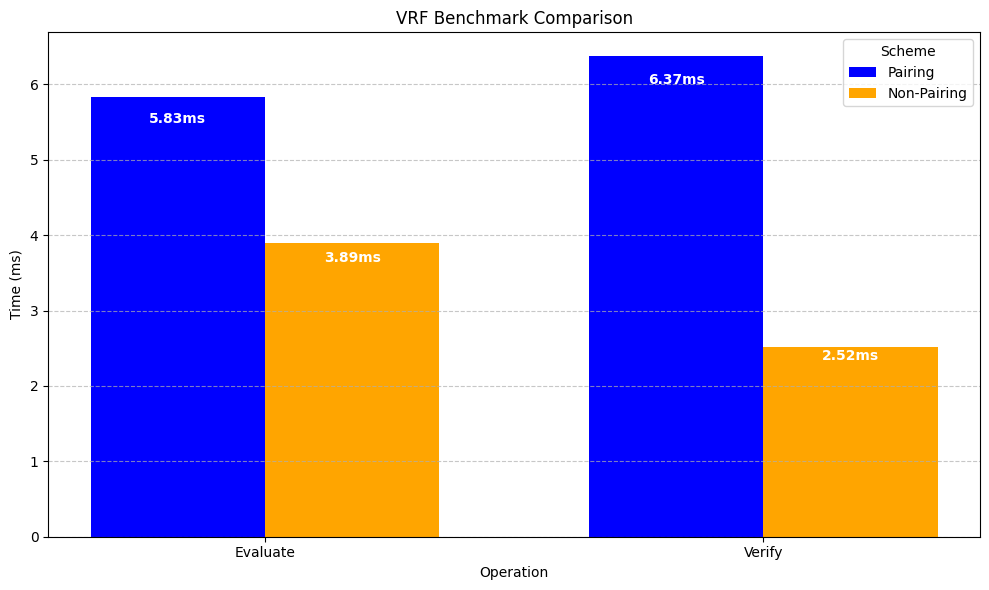
\includegraphics[width=0.75\linewidth]{figures/vrf-benchmark.png}
    \caption{VRF Benchmark}
    \label{fig:vrf-benchmark}
\end{figure}

\clearpage
